\documentclass[10pt]{beamer}
\usepackage[utf8]{inputenc}
\usepackage[T1]{fontenc}
\usetheme{metropolis}
\usepackage{booktabs}
\usepackage[scale=2]{ccicons}
\usepackage{pgfplots}
\usepgfplotslibrary{dateplot}
\usepackage{xspace}
\usepackage{pbox}

% a few macros
\newcommand{\bi}{\begin{itemize}}
\newcommand{\ei}{\end{itemize}}
\newcommand{\ig}{\includegraphics}
\definecolor{hilight}{RGB}{235,129,27}
\definecolor{vhilight}{RGB}{235,129,27}

% title info
\title{Graphs}
\author{Bjarki Ágúst Guðmundsson\\ Tómas Ken Magnússon}
\institute{\href{http://ru.is/td}{School of Computer Science} \\[2pt] \href{http://ru.is}{Reykjavík University}}
\titlegraphic{\hfill\includegraphics[height=0.6cm]{kattis}}
\date{\textbf{Árangursrík forritun og lausn verkefna}}

% Tikz
\usepackage{tikz}
\usetikzlibrary{arrows,shapes}

% Minted
\usepackage{minted}
\usemintedstyle{manni}
\newminted{cpp}{fontsize=\footnotesize}

% Graph styles
\tikzstyle{vertex}=[circle,fill=black!50,minimum size=15pt,inner sep=0pt, font=\small]
\tikzstyle{selected vertex} = [vertex, fill=red!24]
\tikzstyle{edge} = [draw,thick,-]
\tikzstyle{dedge} = [draw,thick,->]
\tikzstyle{weight} = [font=\scriptsize,pos=0.5]
\tikzstyle{selected edge} = [draw,line width=2pt,-,red!50]
\tikzstyle{selected2 vertex} = [vertex, fill=hilight!50, text=black]
\tikzstyle{ignored edge} = [draw,line width=5pt,-,black!20]
\tikzstyle{vertex1} = [vertex, fill=red]
\tikzstyle{vertex2} = [vertex, fill=blue]
\tikzstyle{vertex3} = [vertex, fill=green, text=black]
\tikzstyle{vertex4} = [vertex, fill=yellow, text=black]
\tikzstyle{vertex5} = [vertex, fill=pink, text=black]
\tikzstyle{vertex6} = [vertex, fill=purple]

\tikzset{
  treenode/.style = {align=center, inner sep=0pt, text centered,
    font=\sffamily},
  vertex/.style = {treenode, circle, black, font=\sffamily\bfseries\tiny, draw=black, text width=1.8em},% arbre rouge noir, noeud noir
  rvertex/.style = {treenode, circle, black, font=\sffamily\bfseries\tiny, draw=red, text width=1.8em},% arbre rouge noir, noeud noir
}

\begin{document}
\maketitle

\begin{frame}{Today we're going to cover}
    \bi
        \item Minimum spanning tree
        \item Shortest paths
        % \item Transitive closure
        % \item Minimax/maximin
        \item Some known graph problems
        \item Special graphs
            \bi
                \item Trees
                \item Directed acyclic graphs
                \item Bipartite graphs
            \ei

        % - Minimum spanning tree (and variants)
        % - Shortest path (Dijkstra, Bellman-Ford, Floyd-Warshall)
        % - Transitive closure
        % - Minimax and maximin
        % - Special graphs
        %     - Trees
        %     - DAGs
        %     - Bipartite graphs
    \ei
\end{frame}

% TODO: ...

\begin{frame}{Weighted graphs}
    \bi
        \item Now the edges in our graphs may have weights, which could represent
            \bi
                \item the distance of the road represented by the edge
                \item the cost of going over the edge
                \item some capacity of the edge
            \ei

        \item We can use a modified adjacency list to represent weighted graphs
    \ei
\end{frame}

\begin{frame}[fragile]{Weighted graphs}
    \begin{columns}[T]
        \begin{column}{.4\textwidth}
            \begin{minted}[fontsize=\footnotesize]{cpp}
struct edge {
    int u, v;
    int weight;

    edge(int _u, int _v, int _w) {
        u = _u;
        v = _v;
        weight = _w;
    }
};
            \end{minted}
        \end{column}%
        \hfill%
        \begin{column}{.6\textwidth}
            \begin{figure}
                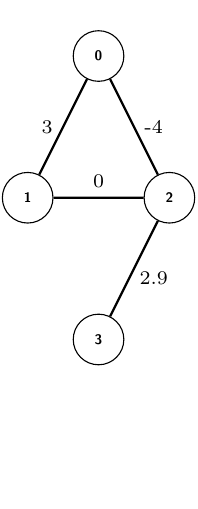
\begin{tikzpicture}[scale=1.8,auto,swap]
                    \node[vertex] (0) at (0.5,3) {0};
                    \node[vertex] (1) at (0,2) {1};
                    \node[vertex] (2) at (1,2) {2};
                    \node[vertex] (3) at (0.5,1) {3};

                    \path[edge] (0) -- node[weight,left] {3} (1);
                    \path[edge] (0) -- node[weight,right] {-4} (2);
                    \path[edge] (1) -- node[weight,above] {0} (2);
                    \path[edge] (2) -- node[weight,right,pos=0.6] {2.9} (3);

                    \pgfresetboundingbox
                    \path [use as bounding box] (0,0) rectangle (1,3.2);
                \end{tikzpicture}
            \end{figure}
        \end{column}%
    \end{columns}
\end{frame}

\begin{frame}[fragile]{Weighted graphs}
    \begin{columns}[T]
        \begin{column}{.4\textwidth}
            \begin{minted}[fontsize=\footnotesize]{cpp}
vector<edge> adj[4];

adj[0].push_back(edge(0, 1, 3));
adj[0].push_back(edge(0, 2, -4));

adj[1].push_back(edge(1, 0, 3));
adj[1].push_back(edge(1, 2, 0));

adj[2].push_back(edge(2, 0, -4));
adj[2].push_back(edge(2, 1, 0));
adj[2].push_back(edge(2, 3, 2.9));

adj[3].push_back(edge(3, 2, 2.9));

            \end{minted}
        \end{column}%
        \hfill%
        \begin{column}{.6\textwidth}
            \begin{figure}
                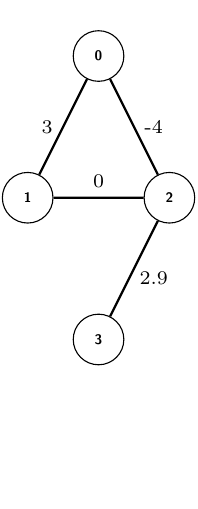
\begin{tikzpicture}[scale=1.8,auto,swap]
                    \node[vertex] (0) at (0.5,3) {0};
                    \node[vertex] (1) at (0,2) {1};
                    \node[vertex] (2) at (1,2) {2};
                    \node[vertex] (3) at (0.5,1) {3};

                    \path[edge] (0) -- node[weight,left] {3} (1);
                    \path[edge] (0) -- node[weight,right] {-4} (2);
                    \path[edge] (1) -- node[weight,above] {0} (2);
                    \path[edge] (2) -- node[weight,right,pos=0.6] {2.9} (3);

                    \pgfresetboundingbox
                    \path [use as bounding box] (0,0) rectangle (1,3.2);
                \end{tikzpicture}
            \end{figure}
        \end{column}%
    \end{columns}
\end{frame}

\begin{frame}{Minimum spanning tree}
    \bi
        \item We have an undirected weighted graph
        \item The vertices along with a subset of the edges in the graph is called a spanning tree if
            \bi
                \item it forms a tree (i.e.\ does not contain a cycle) and
                \item the tree spans all vertices (all vertices can reach all other vertices)
            \ei
        \vspace{10pt}
        \item The weight of a spanning tree is the sum of the weights of the edges in the subset
        \vspace{10pt}
        \item We want to find a minimum spannig tree
    \ei
\end{frame}

\begin{frame}{Minimum spanning tree}
    \bi
        \item Several greedy algorithms work
        \vspace{10pt}
        \item Go through the edges in the graph in increasing order of weight
        \item Greedily pick an edge if it doesn't form a cycle (Union-Find can be used to keep track of when we would get a cycle)
        \item When we've gone through all edges, we have a minimum spanning tree
        \vspace{10pt}
        \item This is Kruskal's algorithm
        \item Time complexity is $O(E \log E)$
    \ei
\end{frame}

\begin{frame}[fragile]{Minimum spanning tree}
    \begin{minted}[fontsize=\scriptsize]{cpp}

bool edge_cmp(const edge &a, const edge &b) {
    return a.weight < b.weight;
}

vector<edge> mst(int n, vector<edge> edges) {
    union_find uf(n);
    sort(edges.begin(), edges.end(), edge_cmp);

    vector<edge> res;
    for (int i = 0; i < edges.size(); i++) {
        int u = edges[i].u,
            v = edges[i].v;

        if (uf.find(u) != uf.find(v)) {
            uf.unite(u, v);
            res.push_back(edges[i]);
        }
    }

    return res;
}
    \end{minted}
\end{frame}

% TODO: Example problem:
% \begin{frame}{Example problem: Dark roads}
%     \bi
%         \item http://uva.onlinejudge.org/external/116/11631.html
%     \ei
% \end{frame}

\begin{frame}{Shortest paths}
    \bi
        \item We have a weighted graph (undirected or directed)
        \item Given two vertices $u,v$, what is the shortest path from $u$ to $v$?
        \vspace{10pt}
        \item If all weights are the same, this can be solved with breadth-first search
        \item Of course, this is usually not the case...
    \ei
\end{frame}

\begin{frame}{Shortest paths}
    \bi
        \item There are many known algorithms to find shortest paths
        \item Like breadth-first search, these algorithms usually find the shortest paths from a given start vertex to all other vertices
        \vspace{5pt}
        \item Let's take a quick look at Dijkstra's algorithm, the Bellman-Ford algorithm and the Floyd-Warshall algorithm
    \ei
\end{frame}

% TODO: Dijkstra's algorithm
% \begin{frame}{Dijkstra's algorithm}
%     \bi
%         \item 
%     \ei
% \end{frame}

\begin{frame}[fragile]{Dijkstra's algorithm}
    \begin{minted}[fontsize=\scriptsize]{cpp}
vector<edge> adj[100];
vector<int> dist(100, INF);

void dijkstra(int start) {
    dist[start] = 0;
    priority_queue<pair<int, int>,
                   vector<pair<int, int> >,
                   greater<pair<int, int> > > pq;
    pq.push(make_pair(dist[start], start));

    while (!pq.empty()) {
        int u = pq.top().second;
        pq.pop();

        for (int i = 0; i < adj[u].size(); i++) {
            int v = adj[u][i].v;
            int w = adj[u][i].weight;

            if (w + dist[u] < dist[v]) {
                dist[v] = w + dist[u];
                pq.push(make_pair(dist[v], v));
            }
        }
    }
}
    \end{minted}
\end{frame}

\begin{frame}{Dijkstra's algorithm}
    \bi
        \item Time complexity is $O(V \log E)$
        \vspace{10pt}
        \item Note that this only works for non-negative weights
    \ei
\end{frame}

% TODO: Bellman-Ford algorithm
\begin{frame}[fragile]{Bellman-Ford algorithm}
    \begin{minted}[fontsize=\footnotesize]{cpp}
void bellman_ford(int n, int start) {

    dist[start] = 0;

    for (int i = 0; i < n - 1; i++) {
        for (int u = 0; u < n; u++) {
            for (int j = 0; j < adj[u].size(); j++) {
                int v = adj[u][j].v;
                int w = adj[u][j].weight;
                dist[v] = min(dist[v], w + dist[u]);
            }
        }
    }
}
    \end{minted}
\end{frame}

\begin{frame}{Bellman-Ford algorithm}
    \bi
        \item Time complexity is $O(V\times E)$
        \vspace{10pt}
        \item Can be used to detect negative-weight cycles
    \ei
\end{frame}

% TODO: Floyd-Warshall algorithm
\begin{frame}{Floyd-Warshall algorithm}
    \bi
        \item What about using dynamic programming to compute shortest paths?
        \vspace{10pt}
    \item Let $\mathrm{sp}(k, i, j)$ be the shortest path from $i$ to $j$ if we're only allowed to travel through the vertices $0$, \ldots, $k$
        \vspace{5pt}
    \item Base case: $\mathrm{sp}(k, i, j) = 0$ if $i = j$
    \item Base case: $\mathrm{sp}(-1, i, j) = \mathrm{weight}[a][b]$ if $(i,j) \in E$
    \item Base case: $\mathrm{sp}(-1, i, j) = \infty$
        \vspace{5pt}
    \item $\mathrm{sp}(k, i, j) = \mathrm{min} \left\{
	\begin{array}{l}
        \mathrm{sp}(k - 1, i, k) + \mathrm{sp}(k - 1, k, j) \\
        \mathrm{sp}(k - 1, i, j)
	\end{array}
\right.$
    \ei
\end{frame}

\begin{frame}[fragile]{Floyd-Warshall algorithm}
    \begin{minted}[fontsize=\scriptsize]{cpp}
int dist[1000][1000];
int weight[1000][1000];

void floyd_warshall(int n) {
    for (int i = 0; i < n; i++) {
        for (int j = 0; j < n; j++) {
            dist[i][j] = i == j ? 0 : weight[i][j];
        }
    }

    for (int k = 0; k < n; k++) {
        for (int i = 0; i < n; i++) {
            for (int j = 0; j < n; j++) {
                dist[i][j] = min(dist[i][j], dist[i][k] + dist[k][j]);
            }
        }
    }
}
    \end{minted}
\end{frame}

\begin{frame}{Floyd-Warshall algorithm}
    \bi
\item Computes all-pairs shortest paths
\item Time complexity is clearly $O(n^3)$
\item Very simple to code
    \ei
\end{frame}

% \begin{frame}{Transitive closure}
% \end{frame}
% 
% \begin{frame}{Minimax/maximin}
% \end{frame}

% TODO: Some common graph problems
\begin{frame}{Known graph problems}
    \bi
        \item The problems we're dealing with very often ask us to solve some well known graph problem
        \item But usually it's well hidden in the problem statement
        \vspace{10pt}
        \item Let's take a look at a few examples
    \ei
\end{frame}

% TODO: Minimum vertex cover
\begin{frame}{Minimum vertex cover}
    \bi
        \item We have an unweighted undirected graph
        \item A vertex cover is a subset of the vertices $S$, such that for each edge $(u, v)$ in the graph, either $u$ or $v$ (or both) are in $S$
    \ei

    \begin{figure}
        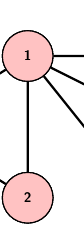
\begin{tikzpicture}[scale=1.8,auto,swap]
            \onslide<1>{
                \node[vertex] (0) at (0,0.5) {0};
                \node[vertex] (1) at (0.8,1) {1};
                \node[vertex] (2) at (0.8,0) {2};
                \node[vertex] (3) at (2,1) {3};
                \node[vertex] (4) at (1.8,0.5) {4};
                \node[vertex] (5) at (1.6,0) {5};
            }
            \onslide<2-3>{
                \node[selected vertex] (0) at (0,0.5) {0};
                \node[selected vertex] (1) at (0.8,1) {1};
                \node[vertex] (2) at (0.8,0) {2};
                \node[vertex] (3) at (2,1) {3};
                \node[selected vertex] (4) at (1.8,0.5) {4};
                \node[vertex] (5) at (1.6,0) {5};
            }
            \onslide<4->{
                \node[vertex] (0) at (0,0.5) {0};
                \node[selected vertex] (1) at (0.8,1) {1};
                \node[selected vertex] (2) at (0.8,0) {2};
                \node[vertex] (3) at (2,1) {3};
                \node[vertex] (4) at (1.8,0.5) {4};
                \node[vertex] (5) at (1.6,0) {5};
            }

            \path[edge] (0) -- (1);
            \path[edge] (0) -- (2);
            \path[edge] (1) -- (2);
            \path[edge] (1) -- (3);
            \path[edge] (1) -- (4);
            \path[edge] (1) -- (5);

            \pgfresetboundingbox
            \path [use as bounding box] (0.8,0) rectangle (1,1.2);
        \end{tikzpicture}
    \end{figure}

    \vspace{10pt}
    \bi
        \item<3-> We want to find a vertex cover of minimum size
        \vspace{10pt}
        \item<5-> NP-hard problem in general graphs
    \ei
\end{frame}

% TODO: Maximum independent set
\begin{frame}{Maximum independent set}
    \bi
        \item We have an unweighted undirected graph
        \item An independent set is a subset of the vertices $S$, such that no two vertices $u,v$ in $S$ are adjacent in the graph
    \ei

    \begin{figure}
        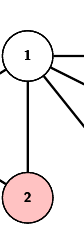
\begin{tikzpicture}[scale=1.8,auto,swap]
            \onslide<1>{
                \node[vertex] (0) at (0,0.5) {0};
                \node[vertex] (1) at (0.8,1) {1};
                \node[vertex] (2) at (0.8,0) {2};
                \node[vertex] (3) at (2,1) {3};
                \node[vertex] (4) at (1.8,0.5) {4};
                \node[vertex] (5) at (1.6,0) {5};
            }
            \onslide<2-3>{
                \node[vertex] (0) at (0,0.5) {0};
                \node[vertex] (1) at (0.8,1) {1};
                \node[selected vertex] (2) at (0.8,0) {2};
                \node[selected vertex] (3) at (2,1) {3};
                \node[vertex] (4) at (1.8,0.5) {4};
                \node[selected vertex] (5) at (1.6,0) {5};
            }
            \onslide<4->{
                \node[selected vertex] (0) at (0,0.5) {0};
                \node[vertex] (1) at (0.8,1) {1};
                \node[vertex] (2) at (0.8,0) {2};
                \node[selected vertex] (3) at (2,1) {3};
                \node[selected vertex] (4) at (1.8,0.5) {4};
                \node[selected vertex] (5) at (1.6,0) {5};
            }

            \path[edge] (0) -- (1);
            \path[edge] (0) -- (2);
            \path[edge] (1) -- (2);
            \path[edge] (1) -- (3);
            \path[edge] (1) -- (4);
            \path[edge] (1) -- (5);

            \pgfresetboundingbox
            \path [use as bounding box] (0.8,0) rectangle (1,1.2);
        \end{tikzpicture}
    \end{figure}

    \vspace{10pt}
    \bi
        \item<3-> We want to find an independent set of maximum size
        \vspace{10pt}
        \item<5-> NP-hard problem in general graphs
    \ei
\end{frame}

\begin{frame}{Relation between MVC and MIS}
    \bi
        \item The previous two problems are very related
        \item A subset of the vertices is a vertex cover if and only if the complement of the set is an independent set
    \ei

    \begin{figure}
        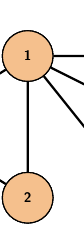
\begin{tikzpicture}[scale=1.8,auto,swap]
            \onslide<1>{
                \node[vertex] (0) at (0,0.5) {0};
                \node[vertex] (1) at (0.8,1) {1};
                \node[vertex] (2) at (0.8,0) {2};
                \node[vertex] (3) at (2,1) {3};
                \node[vertex] (4) at (1.8,0.5) {4};
                \node[vertex] (5) at (1.6,0) {5};
            }
            \onslide<2>{
                \node[selected2 vertex] (0) at (0,0.5) {0};
                \node[selected2 vertex] (1) at (0.8,1) {1};
                \node[selected vertex] (2) at (0.8,0) {2};
                \node[selected vertex] (3) at (2,1) {3};
                \node[selected2 vertex] (4) at (1.8,0.5) {4};
                \node[selected vertex] (5) at (1.6,0) {5};
            }
            \onslide<3->{
                \node[selected vertex] (0) at (0,0.5) {0};
                \node[selected2 vertex] (1) at (0.8,1) {1};
                \node[selected2 vertex] (2) at (0.8,0) {2};
                \node[selected vertex] (3) at (2,1) {3};
                \node[selected vertex] (4) at (1.8,0.5) {4};
                \node[selected vertex] (5) at (1.6,0) {5};
            }

            \path[edge] (0) -- (1);
            \path[edge] (0) -- (2);
            \path[edge] (1) -- (2);
            \path[edge] (1) -- (3);
            \path[edge] (1) -- (4);
            \path[edge] (1) -- (5);

            \pgfresetboundingbox
            \path [use as bounding box] (0.8,0) rectangle (1,1.2);
        \end{tikzpicture}
    \end{figure}

    \vspace{10pt}
    \bi
        \item<4-> The size of a minimum vertex cover plus the size of a maximum independent set is equal to the number of vertices
    \ei
\end{frame}

% TODO: Matching
\begin{frame}{Maximum matching}
    \bi
        \item We have an unweighted undirected graph
        \item A matching is a subset of the edges such that each vertex is adjacent to at most one edge in the subset
    \ei

    \begin{figure}
        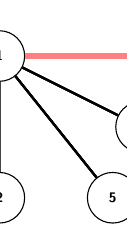
\begin{tikzpicture}[scale=1.8,auto,swap]
            \node[vertex] (0) at (0,0.5) {0};
            \node[vertex] (1) at (0.8,1) {1};
            \node[vertex] (2) at (0.8,0) {2};
            \node[vertex] (3) at (2,1) {3};
            \node[vertex] (4) at (1.8,0.5) {4};
            \node[vertex] (5) at (1.6,0) {5};
            \node[vertex] (6) at (2.4,0) {6};

            \onslide<1>{
                \path[edge] (0) -- (1);
                \path[edge] (0) -- (2);
                \path[edge] (1) -- (2);
                \path[edge] (1) -- (3);
                \path[edge] (1) -- (4);
                \path[edge] (1) -- (5);
                \path[edge] (5) -- (6);
            }
            \onslide<2-3>{
                \path[selected edge] (0) -- (1);
                \path[edge] (0) -- (2);
                \path[edge] (1) -- (2);
                \path[edge] (1) -- (3);
                \path[edge] (1) -- (4);
                \path[edge] (1) -- (5);
                \path[selected edge] (5) -- (6);
            }
            \onslide<4->{
                \path[edge] (0) -- (1);
                \path[selected edge] (0) -- (2);
                \path[edge] (1) -- (2);
                \path[selected edge] (1) -- (3);
                \path[edge] (1) -- (4);
                \path[edge] (1) -- (5);
                \path[selected edge] (5) -- (6);
            }

            \pgfresetboundingbox
            \path [use as bounding box] (1.5,0) rectangle (1,1.2);
        \end{tikzpicture}
    \end{figure}

    \vspace{10pt}
    \bi
        \item<3-> We want to find a matching of maximum size
        \vspace{10pt}
    \item<5-> There exists an $O(V^4)$ algorithm for general graphs, but is pretty complex
    \ei
\end{frame}

% TODO: Coloring
\begin{frame}{Graph coloring}
    \bi
        \item We have an unweighted undirected graph
        \item A coloring of the graph is an assignment of colors to the vertices such that adjacent vertices have different colors
    \ei

    \begin{figure}
        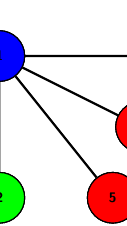
\begin{tikzpicture}[scale=1.8,auto,swap]
            \onslide<1>{
                \node[vertex] (0) at (0,0.5) {0};
                \node[vertex] (1) at (0.8,1) {1};
                \node[vertex] (2) at (0.8,0) {2};
                \node[vertex] (3) at (2,1) {3};
                \node[vertex] (4) at (1.8,0.5) {4};
                \node[vertex] (5) at (1.6,0) {5};
            }
            \onslide<2-3>{
                \node[vertex1] (0) at (0,0.5) {0};
                \node[vertex2] (1) at (0.8,1) {1};
                \node[vertex3] (2) at (0.8,0) {2};
                \node[vertex4] (3) at (2,1) {3};
                \node[vertex5] (4) at (1.8,0.5) {4};
                \node[vertex6] (5) at (1.6,0) {5};
            }
            \onslide<4->{
                \node[vertex1] (0) at (0,0.5) {0};
                \node[vertex2] (1) at (0.8,1) {1};
                \node[vertex3] (2) at (0.8,0) {2};
                \node[vertex1] (3) at (2,1) {3};
                \node[vertex1] (4) at (1.8,0.5) {4};
                \node[vertex1] (5) at (1.6,0) {5};
            }

            \path[edge] (0) -- (1);
            \path[edge] (0) -- (2);
            \path[edge] (1) -- (2);
            \path[edge] (1) -- (3);
            \path[edge] (1) -- (4);
            \path[edge] (1) -- (5);

            \pgfresetboundingbox
            \path [use as bounding box] (1.5,0) rectangle (1,1.2);
        \end{tikzpicture}
    \end{figure}

    \vspace{10pt}
    \bi
        \item<3-> We want to find a coloring that uses the minimum number of distinct colors
        \vspace{10pt}
        \item<5-> NP-hard in general graphs
    \ei

\end{frame}

\begin{frame}{Special graphs}
    \bi
\item All of these problems are hard (in some sense) in general graphs
\item But what if we're working with special kinds of graphs?
    \vspace{10pt}
\item Let's look at a few examples
    \ei
\end{frame}

\begin{frame}{Bipartite graphs}
    \bi
\item A graph is bipartite if the vertices can be partitioned into two sets such that for each edge $(u,v)$ $u$ and $v$ are in different sets
    \ei
    \begin{figure}
        \begin{tikzpicture}[scale=1.8,auto,swap]
            \only<-1>{
                \node[vertex] (0) at (0,0.5) {0};
            }
            \only<2->{
                \node[vertex] (0) at (0,0) {0};
            }
            \node[vertex] (1) at (0.8,1) {1};
            \node[vertex] (2) at (0.8,0) {2};
            \only<-3>{
                \node[vertex] (3) at (2,1) {3};
                \node[vertex] (4) at (1.8,0.5) {4};
                \node[vertex] (5) at (1.6,0) {5};
            }
            \only<4->{
                \node[vertex] (3) at (2,0) {3};
                \node[vertex] (4) at (1.6,0) {4};
                \node[vertex] (5) at (1.2,0) {5};
            }
            \only<-2>{
                \node[vertex] (6) at (0,-0.5) {6};
            }
            \only<3->{
                \node[vertex] (6) at (0,1) {6};
            }

            \path[edge] (0) -- (1);
            \path[edge] (0) -- (6);
            \path[edge] (6) -- (2);
            \path[edge] (1) -- (2);
            \path[edge] (1) -- (3);
            \path[edge] (1) -- (4);
            \path[edge] (1) -- (5);

            \onslide<5->{
                \draw[color=vhilight] (0.4,1) ellipse (0.7cm and 0.3cm);
                \draw[color=vhilight] (1.0,0) ellipse (1.5cm and 0.3cm);
            }

            \pgfresetboundingbox
            \path [use as bounding box] (1.5,0) rectangle (1,1.2);
        \end{tikzpicture}
    \end{figure}

    \vspace{20pt}
    \bi
        \item How do we check if a graph is bipartite?
    \ei
\end{frame}

\begin{frame}{Bipartite graphs}
    \bi
        \item We want to check if we can split the vertices into these two groups
        \item Take any vertex, and assume that it's in the first group
        \item Then all of his neighbors must be in the second group
        \item And then all of their neighbors must be in the first group
        \item And so on...
        \vspace{10pt}
        \item We can do this with a simple depth-first search
        \item If we ever find a contradiction (i.e.\ a vertex must both be in the first and second set), then the graph is not bipartite
    \ei
\end{frame}

\begin{frame}[fragile]{Bipartite graphs}
    \begin{minted}[fontsize=\scriptsize]{cpp}
vector<int> adj[1000];
vector<int> side(1000, -1);
bool is_bipartite = true;

void check_bipartite(int u) {
    for (int i = 0; i < adj[u].size(); i++) {
        int v = adj[u][i];
        if (side[v] == -1) {
            side[v] = 1 - side[u];
            check_bipartite(v);
        } else if (side[u] == side[v]) {
            is_bipartite = false;
        }
    }
}

for (int u = 0; u < n; u++) {
    if (side[u] == -1) {
        side[u] = 0;
        check_bipartite(u);
    }
}
    \end{minted}
\end{frame}

\begin{frame}{Coloring bipartite graphs}
    \bi
        \item What if we want to find the minimum graph coloring of a bipartite graph?
    \ei

    \begin{figure}
        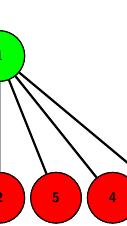
\begin{tikzpicture}[scale=1.8,auto,swap]
            \onslide<-1>{
                \node[vertex] (0) at (0,0) {0};
                \node[vertex] (1) at (0.8,1) {1};
                \node[vertex] (2) at (0.8,0) {2};
                \node[vertex] (3) at (2,0) {3};
                \node[vertex] (4) at (1.6,0) {4};
                \node[vertex] (5) at (1.2,0) {5};
                \node[vertex] (6) at (0,1) {6};
            }
            \onslide<2->{
                \node[vertex1] (0) at (0,0) {0};
                \node[vertex3] (1) at (0.8,1) {1};
                \node[vertex1] (2) at (0.8,0) {2};
                \node[vertex1] (3) at (2,0) {3};
                \node[vertex1] (4) at (1.6,0) {4};
                \node[vertex1] (5) at (1.2,0) {5};
                \node[vertex3] (6) at (0,1) {6};
            }

            \path[edge] (0) -- (1);
            \path[edge] (0) -- (6);
            \path[edge] (6) -- (2);
            \path[edge] (1) -- (2);
            \path[edge] (1) -- (3);
            \path[edge] (1) -- (4);
            \path[edge] (1) -- (5);

            \pgfresetboundingbox
            \path [use as bounding box] (1.5,0) rectangle (1,1.2);
        \end{tikzpicture}
    \end{figure}

    \vspace{20pt}
    \bi
        \item<2-> Simple, one side can be colored with one color, and the second side can be colored with a second color
    \ei
\end{frame}

\begin{frame}{Bipartite matching}
    \bi
        \item Finding a maximum matching in bipartite graphs is very common
        \item \textit{see example}
            \vspace{10pt}
        \item Soon we'll see an efficient algorithm for finding the maximum matching in a bipartite graph
    \ei
\end{frame}

\begin{frame}{König's theorem}
    \bi
        \item König's theorem states that the size of a minimum vertex cover in a bipartite graph is equal to the size of the maximum matching in that graph
        \vspace{10pt}
        \item To find the minimum vertex cover in a bipartite graph, we just find the maximum matching with our efficient algorithm, and we have our answer
        \item And since the size of the maximum independent set is just the number of vertices minus the size of the minimum vertex cover, we can also compute the maximum independent set for a bipartite graph efficiently
    \ei
\end{frame}

\begin{frame}{Trees}
    \bi
\item An undirected graph is a tree if it has no cycles
    \vspace{10pt}
\item Easy to check if a graph is a tree by checking if there are any backward edges in the depth-first search tree (see previous lecture)
\vspace{10pt}
\item A connected tree with $n$ vertices has exactly $n-1$ edges
\vspace{10pt}
\item Between each pair of vertices $u,v$ in the tree, there exists exactly one simple path, which can be found with depth-first search (or breadth-first search)
    \ei
\end{frame}

\begin{frame}{Trees}
    \bi
\item What if we look at these problems for trees?
    \vspace{10pt}
\item How do we find the minimum number of colors needed to color a tree?

    \onslide<2->{
        \vspace{10pt}
        \item Well, trees are actually bipartite graphs...
        \item Why? Pick some vertex and make it the root of the tree. Then vertices at even heights in the tree can be put on one side, and vertices at odd heights can be put on the other side
        \vspace{10pt}
        \item So all the efficient algorithms for bipartite graphs also work for trees
    }
    \ei
\end{frame}

\begin{frame}{Trees}
    \bi
        \item Trees are also well suited for dynamic programming, so many problems become simpler here because of that
    \ei
\end{frame}

\begin{frame}{Directed acyclic graphs}
    \bi
        \item A directed graph is a directed acyclic graph if it doesn't contain any cycles
    \vspace{10pt}
\item Easy to check if a graph is a DAG by checking if there are any backward edges in the depth-first search tree (see previous lecture)
    \vspace{10pt}
\item Many problems are simple on DAGs, since it's easy to do dynamic programming over DAGs
        \bi
            \item counting number of simple paths from $u$ to $v$
            \item longest simple path from $u$ to $v$
        \ei
    \ei
\end{frame}

\end{document}

